% ============================================================
%  ChiangMai Air Quality Alert System — Project Proposal
%  AIT Course AT82.9002 | Selected Topic: Data Engineering and MLOps
%  Authors: Supanut Komolvanij (st126055), Shuvam Shrestha (st125975)
% ============================================================

\documentclass[12pt,a4paper]{report}

% ---- Encoding & Fonts ----
\usepackage[utf8]{inputenc}
\usepackage[T1]{fontenc}
\usepackage{times}                    % Times New Roman (AIT standard)

% ---- Page Layout ----
\usepackage[
  top=1in, bottom=1in,
  left=1.5in, right=1in            % AIT binding margin
]{geometry}
\usepackage{setspace}
\onehalfspacing                      % AIT: 1.5 line spacing throughout

% ---- Typography & Headings ----
\usepackage{titlesec}
\usepackage{parskip}
\setlength{\parindent}{0pt}
\setlength{\parskip}{6pt}

% Chapter: centered, all-caps, bold
\titleformat{\chapter}[display]
  {\normalfont\large\bfseries\centering}
  {\MakeUppercase{\chaptertitlename}\ \thechapter}
  {0pt}
  {\large\MakeUppercase}
\titlespacing*{\chapter}{0pt}{-10pt}{24pt}

% Section
\titleformat{\section}
  {\normalfont\normalsize\bfseries}{\thesection}{1em}{}
\titlespacing*{\section}{0pt}{12pt}{6pt}

% Subsection
\titleformat{\subsection}
  {\normalfont\normalsize\bfseries}{\thesubsection}{1em}{}
\titlespacing*{\subsection}{0pt}{10pt}{4pt}

% Subsubsection
\titleformat{\subsubsection}
  {\normalfont\normalsize\itshape}{\thesubsubsection}{1em}{}
\titlespacing*{\subsubsection}{0pt}{8pt}{2pt}

% ---- Tables ----
\usepackage{booktabs}
\usepackage{longtable}
\usepackage{array}
\usepackage{multirow}
\usepackage{tabularx}
\renewcommand{\arraystretch}{1.3}

% ---- Figures & Floats ----
\usepackage{graphicx}
\usepackage{float}
\usepackage{caption}
\usepackage{subcaption}
\usepackage{tikz}
\usetikzlibrary{shapes.geometric, arrows.meta, positioning, fit, backgrounds}

% ---- Math ----
\usepackage{amsmath}
\usepackage{amssymb}

% ---- Lists ----
\usepackage{enumitem}
\setlist[itemize]{topsep=4pt, itemsep=2pt}
\setlist[enumerate]{topsep=4pt, itemsep=2pt}

% ---- Code Listings ----
\usepackage{listings}
\usepackage{xcolor}
\lstset{
  basicstyle=\small\ttfamily,
  breaklines=true,
  frame=single,
  backgroundcolor=\color{gray!8},
  keywordstyle=\color{blue!70},
  commentstyle=\color{green!55!black},
  stringstyle=\color{red!60!black},
  numbers=left,
  numberstyle=\tiny\color{gray},
  xleftmargin=1.5em
}

% ---- Headers & Footers ----
\usepackage{fancyhdr}
\pagestyle{fancy}
\fancyhf{}
\fancyhead[R]{\thepage}
\renewcommand{\headrulewidth}{0pt}
\fancypagestyle{plain}{%
  \fancyhf{}
  \fancyhead[R]{\thepage}
  \renewcommand{\headrulewidth}{0pt}
}

% ---- Table of Contents ----
\usepackage{tocloft}
\renewcommand{\cfttoctitlefont}{\large\bfseries}
\renewcommand{\cftloftitlefont}{\large\bfseries}
\renewcommand{\cftlottitlefont}{\large\bfseries}

% ---- Hyperlinks ----
\usepackage[
  colorlinks=true,
  linkcolor=black,
  citecolor=black,
  urlcolor=blue!70!black,
  bookmarks=true
]{hyperref}
\usepackage{url}

% ---- Placeholder figure box ----
\newcommand{\figplaceholder}[3][14]{%
  % #1 = width in cm (default 14), #2 = height in cm, #3 = label text
  \begin{figure}[H]
    \centering
    \begin{tikzpicture}
      \draw[dashed, thick, gray!55, rounded corners=4pt]
        (0,0) rectangle (#1,#2);
      \node[gray!70, font=\small\itshape, align=center] at (#1/2,#2/2)
        {#3};
    \end{tikzpicture}
  \end{figure}
}

% ============================================================
\begin{document}
% ============================================================

% ---- Roman numerals for front matter ----
\pagenumbering{roman}

% ============================================================
%  TITLE PAGE
% ============================================================
\begin{titlepage}
\begin{center}
\vspace*{1.5cm}

{\large\bfseries CHIANGMAI AIR QUALITY ALERT SYSTEM: \\[0.4em]
END-TO-END MLOPS PIPELINE FOR PM2.5 FORECASTING}

\vspace{2.5cm}

by

\vspace{1.2cm}

{\normalsize
Supanut Kompayak (st126055) \\[0.4em]
Shuvam Shrestha (st125975)
}

\vspace{2.2cm}

\begin{spacing}{1.5}
{\normalsize
A Project Proposal Submitted in Partial Fulfillment of the Requirements \\
for the Course AT82.9002 -- Selected Topic: Data Engineering and MLOps
}
\end{spacing}

\vspace{1.5cm}

\begin{tabular}{ll}
  Instructor:   & Dr.\ Chantri Polprasert \\[0.4em]
  Course:       & AT82.9002 Selected Topic: Data Engineering and MLOps \\[0.4em]
  Semester:     & January 2026 \\
\end{tabular}

\vfill

Asian Institute of Technology \\
School of Engineering and Technology \\
Thailand \\[0.4em]
March 2026

\end{center}
\end{titlepage}

% ============================================================
%  ABSTRACT
% ============================================================
\chapter*{ABSTRACT}
\addcontentsline{toc}{chapter}{ABSTRACT}

Chiang Mai, Thailand, consistently ranks among the most severely air-polluted cities in the world during its annual haze season from January to April. Fine particulate matter (PM2.5) regularly exceeds the World Health Organization's 24-hour guideline of 15~\textmu g/m\textsuperscript{3} by a factor of three or more, posing significant respiratory and cardiovascular health risks to residents, tourists, and vulnerable populations. Despite the severity and predictability of these pollution episodes, existing public-facing tools provide only real-time monitoring with no forward-looking predictive capability.

This proposal presents the ChiangMai Air Quality Alert System (CAAS), a production-ready end-to-end MLOps pipeline that forecasts PM2.5 concentration levels 1, 3, and 7 days in advance and automatically triggers health alerts when projected concentrations exceed the 50~\textmu g/m\textsuperscript{3} hazardous threshold. The system integrates three complementary data sources: historical and real-time PM2.5 observations from Thailand's Pollution Control Department (PCD) monitoring network, meteorological variables from the Open-Meteo API, and fire hotspot detections from NASA FIRMS. A 15-year dataset spanning 2011 to 2025 (approximately 5,475 daily observations) forms the training foundation.

The proposed methodology employs a two-model comparative strategy. An XGBoost model, augmented by 44 engineered temporal and contextual features, serves as the primary baseline and is expected to perform strongly across all horizons given its well-documented efficiency on moderate-sized tabular data. A Long Short-Term Memory (LSTM) network with a 30-day input window is deployed as a comparative sequential model to empirically test whether explicit sequence modeling provides additional forecasting benefit, particularly at longer horizons (t+3, t+7). The selection of the production model will be determined by empirical evaluation rather than assumed in advance.

The MLOps infrastructure is designed for reliability and maintainability, featuring automated daily batch ingestion orchestrated by GitHub Actions, AWS cloud deployment (S3, Lambda, EC2), experiment tracking via MLflow, data drift monitoring via Evidently AI, and automated retraining triggers. The estimated deployment cost is less than \$8 per month in cloud resources.

\newpage

% ============================================================
%  TABLE OF CONTENTS
% ============================================================
\tableofcontents
\newpage

% ============================================================
%  LIST OF TABLES
% ============================================================
\listoftables
\newpage

% ============================================================
%  LIST OF FIGURES
% ============================================================
\listoffigures
\newpage

% ============================================================
%  LIST OF ABBREVIATIONS
% ============================================================
\chapter*{LIST OF ABBREVIATIONS}
\addcontentsline{toc}{chapter}{LIST OF ABBREVIATIONS}

\begin{tabular}{@{}ll}
  API    & Application Programming Interface \\
  AQI    & Air Quality Index \\
  AWS    & Amazon Web Services \\
  CAAS   & ChiangMai Air Quality Alert System \\
  CI/CD  & Continuous Integration / Continuous Deployment \\
  EC2    & Elastic Compute Cloud (AWS) \\
  FIRMS  & Fire Information for Resource Management System \\
  FRP    & Fire Radiative Power \\
  LSTM   & Long Short-Term Memory \\
  MAE    & Mean Absolute Error \\
  ML     & Machine Learning \\
  MLOps  & Machine Learning Operations \\
  PCD    & Pollution Control Department (Thailand) \\
  PM2.5  & Particulate Matter with diameter $\leq$2.5~\textmu m \\
  PSI    & Population Stability Index \\
  REST   & Representational State Transfer \\
  RMSE   & Root Mean Squared Error \\
  S3     & Amazon Simple Storage Service \\
  SHAP   & SHapley Additive exPlanations \\
  WHO    & World Health Organization \\
\end{tabular}

\newpage

% ---- Switch to Arabic numerals for main body ----
\pagenumbering{arabic}

% ============================================================
%  CHAPTER 1 — INTRODUCTION
% ============================================================
\chapter{INTRODUCTION}

\section{Background of the Study}

Air quality degradation from fine particulate matter (PM2.5) represents one of the most pressing environmental health challenges in Southeast Asia. PM2.5 particles, with aerodynamic diameters of 2.5 micrometers or less, penetrate deep into the respiratory system and are associated with increased incidence of respiratory disease, cardiovascular disease, and premature mortality~\cite{who2021}. The World Health Organization's revised 2021 air quality guidelines set the 24-hour mean PM2.5 threshold at 15~\textmu g/m\textsuperscript{3}---a standard that Chiang Mai regularly exceeds by a factor of three to six during its haze season.

Chiang Mai's air quality crisis is driven by a convergence of factors: agricultural burning in the lowlands, wildfires in the surrounding highland forests, transboundary smoke from neighbouring countries (notably Myanmar and Laos), and the city's basin-shaped topography, which limits atmospheric dispersion and traps pollutants near the ground. These conditions create highly predictable annual pollution cycles, with peak concentrations typically occurring between January and April, punctuated by acute events triggered by concentrated fire activity.

Despite the predictability of these patterns, the public information infrastructure remains reactive rather than proactive. Thailand's PCD provides real-time AQI data through the air4thai platform, but no operational system exists to forecast upcoming pollution levels or automatically alert residents and health authorities before dangerous thresholds are breached. The resulting gap between available observational data and actionable early warning represents both a significant public health failure and a data engineering opportunity with real societal impact.

\section{Statement of the Problem}

The core problem addressed by this project is the absence of a predictive, automated early warning system for PM2.5 air quality events in Chiang Mai. Current tools inform the public about pollution that has already occurred; they cannot provide advance notice of conditions likely to develop over the coming one to seven days.

Specifically, the following capability gaps exist in the current landscape:
\begin{enumerate}
  \item No operational system predicts PM2.5 concentration levels 1, 3, or 7~days in advance for Chiang Mai or Northern Thailand more broadly.
  \item No automated mechanism exists to trigger health alerts before PM2.5 reaches hazardous thresholds, denying residents and public health agencies the lead time needed for protective action.
  \item No self-updating system adapts to the shifting pollution patterns driven by changing agricultural practices, increasing wildfire frequency, and long-term climate trends.
\end{enumerate}

\begin{table}[H]
\centering
\caption{Problem framing summary}
\label{tab:problem_framing}
\begin{tabular}{@{}lp{9.5cm}@{}}
\toprule
\textbf{Dimension} & \textbf{Description} \\
\midrule
Who is affected    & Residents, tourists, public health agencies, city planners \\[4pt]
Core problem       & No predictive early warning system exists---only real-time monitoring \\[4pt]
Impact             & Preventable health exposure due to lack of advance notice \\[4pt]
Gap                & Existing tools show current conditions; none forecast what is coming \\[4pt]
Proposed solution  & End-to-end MLOps pipeline: daily forecast (t+1/3/7) + automated alert + drift-aware retraining \\
\bottomrule
\end{tabular}
\end{table}

\section{Objectives of the Study}

The primary objective of this project is to design and implement a production-ready MLOps pipeline providing accurate PM2.5 forecasts and automated health alerts for Chiang Mai. The specific objectives are:

\begin{enumerate}
  \item To design and implement a multi-source data ingestion pipeline that automatically collects PM2.5, weather, and fire hotspot data on a daily basis.
  \item To engineer a feature set capturing temporal autocorrelation, seasonal patterns, meteorological influences, and regional fire activity signals.
  \item To train and empirically compare XGBoost and LSTM models for PM2.5 regression and alert classification across multiple forecast horizons (t+1, t+3, t+7).
  \item To deploy the forecasting system as a REST API and Streamlit dashboard accessible to end users.
  \item To implement a monitoring and automated retraining system detecting data drift and model performance degradation using Evidently AI and MLflow.
  \item To demonstrate a cost-effective cloud deployment within AWS Learner Lab constraints (\$2--8/month target).
\end{enumerate}

\section{Organization of the Report}

Chapter~2 reviews relevant background literature on PM2.5 forecasting, time series modeling, and MLOps principles. Chapter~3 describes the proposed methodology including data pipeline design, feature engineering, and model selection rationale. Chapter~4 details the system architecture and full MLOps lifecycle. Chapter~5 presents the experimental design, evaluation plan, expected contributions, and project timeline.

% ============================================================
%  CHAPTER 2 — BACKGROUND AND RELATED WORK
% ============================================================
\chapter{BACKGROUND AND RELATED WORK}

\section{PM2.5 Air Pollution and Public Health}

Fine particulate matter (PM2.5) is among the most comprehensively studied environmental health hazards globally. Long-term epidemiological evidence demonstrates statistically robust associations between PM2.5 exposure and respiratory disease, ischemic heart disease, stroke, and lung cancer~\cite{who2021}. The WHO 2021 Global Air Quality Guidelines tightened the 24-hour PM2.5 guideline from 25~\textmu g/m\textsuperscript{3} to 15~\textmu g/m\textsuperscript{3}, reflecting accumulated evidence of health impacts at lower concentrations than previously understood.

Northern Thailand's haze problem is characterised by sharp seasonal spikes driven primarily by biomass burning. Unlike urban vehicular pollution, which tends to be geographically diffuse and temporally consistent, fire-driven PM2.5 episodes are spatially concentrated and temporally clustered. This structure makes them, in principle, predictable from fire activity and meteorological precursors---a property that motivates the data-driven forecasting approach in this project.

\section{Data-Driven Approaches for Air Quality Forecasting}

Traditional approaches to air quality forecasting rely on physics-based chemical transport models (CTMs) such as WRF-Chem and CMAQ, which simulate atmospheric dynamics and chemistry explicitly~\cite{seinfeld2016}. While physically interpretable, these models are computationally intensive, require detailed emission inventories, and are difficult to adapt to local conditions without domain expertise.

Data-driven machine learning approaches have increasingly demonstrated competitive performance for short-range air quality forecasting, particularly when rich observational histories are available. Gradient boosting methods such as XGBoost and LightGBM perform strongly on tabular time series when temporal lag features are included, effectively encoding the autoregressive structure of pollution time series into a flat feature representation~\cite{chen2016xgboost}. Studies in regional PM2.5 forecasting in China, India, and Southeast Asia report $R^2$ values in the range of 0.70--0.88 for next-day prediction using similar feature engineering approaches~\cite{liang2020}.

\section{Tabular Models versus Sequential Models for Time Series}

The relative merits of gradient boosting methods and deep sequential models (LSTM, Transformer) for tabular time series prediction have been an active area of benchmarking research. The M4 and M5 forecasting competitions demonstrated that tree-based and statistical ensemble methods consistently match or outperform deep learning approaches across a wide range of time series domains~\cite{makridakis2018m4}.

Shwartz-Ziv and Armon~\cite{shwartzziv2022tabular} conducted a systematic evaluation demonstrating that gradient boosting methods (XGBoost, CatBoost) generally outperform deep learning on tabular datasets with moderate sample sizes, particularly when domain-relevant features are explicitly engineered. Their findings are directly relevant to the dataset considered in this project: approximately 5,475 daily observations is a moderate-size tabular dataset by machine learning standards.

Hochreiter and Schmidhuber's Long Short-Term Memory architecture~\cite{hochreiter1997lstm} was designed specifically to capture long-range temporal dependencies without the vanishing gradient problem of standard RNNs. LSTM has demonstrated advantages over tabular models in domains where the \textit{sequence itself} contains information beyond what fixed-window lag features can encode---for example, in multi-step forecasting tasks where the future trajectory depends on complex interactions across long lookback periods.

\textbf{Implication for this project:} Given the dataset size and the fact that the feature engineering strategy already encodes autocorrelation explicitly through lag and rolling features, XGBoost is expected to perform well across all forecast horizons. LSTM is included as a comparative model to empirically test whether sequential modeling provides additional benefit---particularly at t+3 and t+7 horizons where fixed-lag features may capture less of the relevant dynamics. The production model selection will be determined by empirical evidence, not assumed in advance.

\section{MLOps: Principles and Tools}

MLOps is the practice of applying DevOps principles to machine learning systems to enable reliable, scalable, and maintainable deployment of ML models in production. Sculley et al.~\cite{sculley2015} identified the pervasive challenge of ``hidden technical debt'' in ML systems, noting that the model training code typically represents only a small fraction of total system complexity, with data pipelines, serving infrastructure, and monitoring comprising the majority of the codebase and operational burden.

Key operational challenges in production ML systems include: data distribution shift (data drift) causing model predictions to degrade over time, concept drift where the statistical relationship between inputs and targets changes, and the need for reproducible experiment tracking to enable model comparison and rollback~\cite{sculley2015}.

This project addresses these challenges through a combination of MLflow for experiment tracking and model registry management~\cite{zaharia2018mlflow}, Evidently AI for automated drift detection, and GitHub Actions for CI/CD orchestration. The combination of these tools provides a lightweight but complete MLOps stack appropriate for the project scope and budget constraints.

\section{Related Systems and Novelty}

Thailand's PCD air4thai platform~\cite{pcd2024} provides real-time AQI data from approximately 90 monitoring stations nationwide but offers no forecasting capability. NASA FIRMS~\cite{firms2024} provides near-real-time global fire detection data from MODIS and VIIRS satellite instruments, enabling quantification of fire activity as an explanatory variable for PM2.5 episodes. Open-Meteo~\cite{openmeteo2023} provides free retrospective and forecast meteorological data suitable for academic applications.

No published operational system to date combines these three data sources into an automated daily forecasting and alerting pipeline for Chiang Mai. The primary novelty of CAAS lies in integrating multi-source data acquisition, feature engineering, ML model training and comparison, automated deployment, and continuous monitoring within a single production-grade pipeline aligned with current MLOps best practices.

% ============================================================
%  CHAPTER 3 — PROPOSED METHODOLOGY
% ============================================================
\chapter{PROPOSED METHODOLOGY}

\section{System Overview}

The ChiangMai Air Quality Alert System (CAAS) is designed as a fully automated end-to-end MLOps pipeline. The system ingests data from three sources daily, generates PM2.5 regression forecasts and binary alert classifications for the next 1, 3, and 7~days, and triggers automated health alerts when concentrations are projected to exceed the 50~\textmu g/m\textsuperscript{3} threshold. A monitoring subsystem continuously evaluates forecast accuracy and detects data drift, triggering automated retraining when degradation is detected.

\begin{figure}[H]
\centering
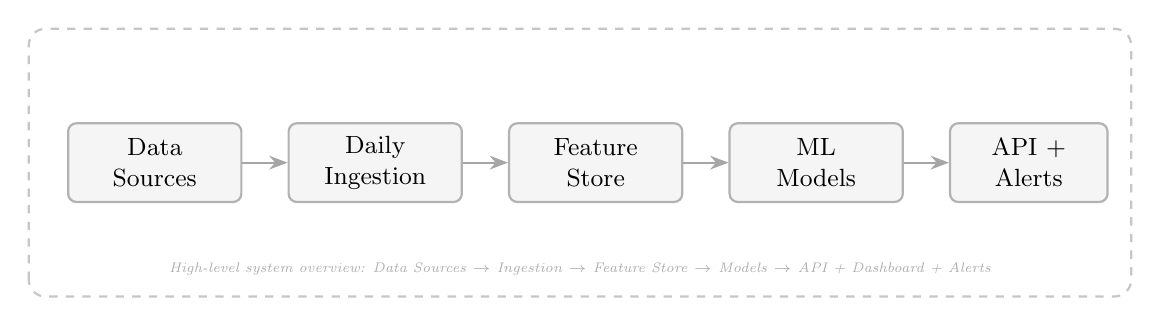
\begin{tikzpicture}[
  box/.style={rectangle, rounded corners=3pt, draw=gray!60, thick,
              fill=gray!8, font=\small, align=center, minimum height=1cm},
  arr/.style={->, >=Stealth, thick, gray!70}
]
  \draw[dashed, thick, gray!45, rounded corners=6pt] (-0.5,-0.7) rectangle (13.5,2.7);
  \node[gray!65, font=\tiny\itshape] at (6.5,-0.35)
        {High-level system overview: Data Sources $\to$ Ingestion $\to$ Feature Store $\to$ Models $\to$ API + Dashboard + Alerts};
  \node[box, minimum width=2.2cm] (src)  at (1.1,1)    {Data\\Sources};
  \node[box, minimum width=2.2cm] (ing)  at (3.9,1)    {Daily\\Ingestion};
  \node[box, minimum width=2.2cm] (feat) at (6.7,1)    {Feature\\Store};
  \node[box, minimum width=2.2cm] (mod)  at (9.5,1)    {ML\\Models};
  \node[box, minimum width=2.0cm] (out)  at (12.2,1)   {API +\\Alerts};
  \draw[arr] (src) -- (ing);
  \draw[arr] (ing) -- (feat);
  \draw[arr] (feat) -- (mod);
  \draw[arr] (mod) -- (out);
\end{tikzpicture}
\caption{High-level overview of the ChiangMai Air Quality Alert System (CAAS).}
\label{fig:system_overview}
\end{figure}

\section{Data Pipeline Design}

\subsection{Data Sources}

The pipeline integrates three data sources, each providing a distinct signal relevant to PM2.5 forecasting in Northern Thailand.

\begin{table}[H]
\centering
\caption{Summary of integrated data sources}
\label{tab:data_sources}
\begin{tabularx}{\textwidth}{@{}p{3cm}p{3cm}p{2cm}X@{}}
\toprule
\textbf{Source} & \textbf{Provider} & \textbf{Type} & \textbf{Coverage \& Granularity} \\
\midrule
PM2.5 concentration & air4thai / PCD Thailand & Excel + REST API & 2011--2025, stations 35T \& 36T, Chiang Mai (daily average) \\[4pt]
Historical weather   & Open-Meteo API          & REST API         & Chiang Mai coordinates (daily) \\[4pt]
Fire hotspots        & NASA FIRMS API          & REST API         & Northern Thailand bounding box (daily) \\
\bottomrule
\end{tabularx}
\end{table}

The primary station is 35T (Chiang Mai City Hall, Chang Phueak), with station 36T (Yupparaj School, Si Phum) serving as a fallback during gaps. The two stations exhibit a Pearson correlation of $r = 0.94$, confirming 36T as a reliable substitute for short-duration absences at the primary station. The full training dataset comprises approximately 5,475 daily observations spanning 15 years.

\subsection{Ingestion Method}

Data ingestion follows a two-mode strategy. A one-time historical load parses all 15 PCD Excel files (one per year, 2011--2025) to build the initial training corpus. Ongoing ingestion runs daily at 06:00 local time via a scheduled GitHub Actions workflow, retrieving the previous day's data from all three sources before executing the forecast pipeline.

Batch ingestion (rather than streaming) is appropriate for this use case because daily forecast granularity provides no operational benefit from sub-hourly data updates.

\subsection{Transformation Pipeline}

Transformations are applied in the following order within each pipeline execution:

\begin{enumerate}
  \item \textbf{Schema validation} --- verify expected columns, data types, and valid date range; pipeline halts immediately on any violation with no silent failures.
  \item \textbf{Missing value handling} --- interpolate PM2.5 gaps of up to three consecutive days using lag and rolling mean; substitute 36T station data for longer gaps; set fire count to zero on days with no detected hotspots.
  \item \textbf{Unit normalisation} --- standardise column names, numeric types, and date formats across all three source schemas.
  \item \textbf{Feature engineering} --- compute all derived features as described in Section~3.3.
  \item \textbf{Target variable creation} --- generate PM2.5 forward-shifted targets for $t+1$, $t+3$, and $t+7$.
\end{enumerate}

Orchestration is managed by GitHub Actions (cron: \texttt{0 6 * * *}). Each step logs success or failure explicitly, and checkpoints are saved after each step to enable pipeline resumption without re-running from scratch.

\section{Feature Engineering}

The full feature set comprises 44 engineered features organised into two groups: temporal autocorrelation features and contextual environmental features.

\subsection{Temporal Features}

\begin{table}[H]
\centering
\caption{Temporal autocorrelation and calendar features}
\label{tab:temporal_features}
\begin{tabularx}{\textwidth}{@{}lX@{}}
\toprule
\textbf{Feature} & \textbf{Description} \\
\midrule
\texttt{PM25\_lag1/2/3/7/14}       & PM2.5 values 1--14~days prior; captures short-term autocorrelation \\
\texttt{PM25\_roll3/7/14/30\_mean} & Rolling mean over 3--30~day windows; captures medium-term trend \\
\texttt{PM25\_roll7/30\_std}       & Rolling standard deviation; quantifies pollution volatility \\
\texttt{month\_sin}, \texttt{month\_cos} & Cyclical month encoding; avoids ordinality assumption \\
\texttt{day\_sin}, \texttt{day\_cos}     & Cyclical day-of-year encoding \\
\texttt{is\_haze\_season}          & Binary: 1 if January--April \\
\texttt{is\_rainy\_season}         & Binary: 1 if May--October \\
\texttt{is\_cool\_season}          & Binary: 1 if November--December \\
\bottomrule
\end{tabularx}
\end{table}

\subsection{Contextual Environmental Features}

\begin{table}[H]
\centering
\caption{Contextual meteorological and fire activity features}
\label{tab:contextual_features}
\begin{tabularx}{\textwidth}{@{}lX@{}}
\toprule
\textbf{Feature} & \textbf{Description} \\
\midrule
\texttt{north\_avg\_PM25}       & Average PM2.5 across 15 Northern Thailand stations; regional smoke signal \\
\texttt{north\_max\_PM25}       & Maximum PM2.5 across Northern Thailand stations \\
\texttt{wind\_speed}, \texttt{wind\_dir} & Wind speed and direction from Open-Meteo; governs smoke transport \\
\texttt{humidity}, \texttt{temperature} & Atmospheric conditions from Open-Meteo \\
\texttt{boundary\_layer\_height}        & Atmospheric mixing height; key driver of surface PM2.5 accumulation \\
\texttt{fire\_count}             & Daily hotspot count within 100~km of Chiang Mai (NASA FIRMS) \\
\texttt{fire\_frp\_sum}          & Total Fire Radiative Power; proxy for fire intensity and smoke volume \\
\bottomrule
\end{tabularx}
\end{table}

\subsection{Target Variables}

\begin{table}[H]
\centering
\caption{Target variables for regression and classification tasks}
\label{tab:targets}
\begin{tabular}{@{}llp{7cm}@{}}
\toprule
\textbf{Variable}    & \textbf{Type}              & \textbf{Definition} \\
\midrule
\texttt{PM25\_next1} & Regression                 & PM2.5 concentration tomorrow (\textmu g/m\textsuperscript{3}) \\
\texttt{PM25\_next3} & Regression                 & PM2.5 concentration in 3~days \\
\texttt{PM25\_next7} & Regression                 & PM2.5 concentration in 7~days \\
\texttt{alert\_next1}& Binary classification      & 1 if PM2.5 tomorrow $>$ 50~\textmu g/m\textsuperscript{3} \\
\texttt{alert\_next3}& Binary classification      & 1 if PM2.5 in 3~days $>$ 50~\textmu g/m\textsuperscript{3} \\
\bottomrule
\end{tabular}
\end{table}

\section{Model Training and Evaluation}

\subsection{Model Selection Rationale}

This project employs a two-model comparative strategy rather than assuming \textit{a priori} that one architecture will outperform the other. This decision is motivated by an important consideration raised during proposal review: with approximately 5,475 daily observations, does a sequential deep learning model offer genuine advantages over a well-tuned gradient boosting model with rich temporal features?

The honest answer is: not necessarily. The comparative experimental design allows the data to answer this question empirically.

\subsubsection{XGBoost --- Primary Baseline Model}

XGBoost~\cite{chen2016xgboost} is the primary baseline and a strong candidate for the production model. Its key advantages for this dataset include:
\begin{itemize}
  \item Efficient and robust training on moderate-sized tabular data with limited overfitting risk.
  \item Native handling of missing values without imputation.
  \item Strong regularisation (L1/L2) to prevent overfitting on the approximately 5,475-sample training set.
  \item Interpretability via SHAP feature importance analysis, enabling model behaviour explanation to non-technical stakeholders.
  \item Given that the temporal features already encode autocorrelation and rolling patterns explicitly, XGBoost operates on a feature representation that has effectively ``pre-digested'' the sequence structure into a flat tabular form---which is precisely where gradient boosting excels.
\end{itemize}

\subsubsection{LSTM --- Comparative Sequential Model}

An LSTM network~\cite{hochreiter1997lstm} with a 30-day input window is deployed as a comparative sequential model. The rationale for including LSTM is not an expectation of across-the-board superiority, but a specific testable hypothesis:

\textbf{Hypothesis:} XGBoost is expected to perform strongly on t+1 forecasting, where the lag-1 feature is highly predictive and the fixed-window feature representation is adequate. LSTM may demonstrate advantages on longer-horizon forecasts (t+3, t+7), where multi-step sequential dependencies and the compounding of seasonal atmospheric signals may be better captured through explicit sequence modelling than through the static lag features available to XGBoost.

Regarding the sample size: while the dataset contains approximately 5,475 row-level observations, training an LSTM with a 30-day sliding window generates approximately 5,400 overlapping sequence samples of length 30. Regularisation measures including dropout (rate 0.2--0.3), L2 weight decay, and early stopping will be applied to mitigate overfitting risk. If LSTM training proves unstable or overfitting cannot be controlled, the XGBoost model will serve as the sole production model---a fully acceptable outcome since the comparative evaluation is itself the contribution.

\subsection{Chronological Data Split}

A strict chronological split is used with no data shuffling, respecting the temporal dependency structure and simulating realistic deployment conditions.

\begin{table}[H]
\centering
\caption{Chronological training, validation, and test split}
\label{tab:data_split}
\begin{tabular}{@{}llp{8.5cm}@{}}
\toprule
\textbf{Split} & \textbf{Period} & \textbf{Rationale} \\
\midrule
Training   & 2011--2022 & 12 years; includes multiple complete haze seasons \\
Validation & 2023       & Hyperparameter tuning; one complete annual cycle \\
Test       & 2024--2025 & Fully unseen; includes the most recent haze seasons \\
\bottomrule
\end{tabular}
\end{table}

% ============================================================
%  CHAPTER 4 — SYSTEM ARCHITECTURE
% ============================================================
\chapter{SYSTEM ARCHITECTURE AND PIPELINE DESIGN}

\section{Architecture Overview}

The CAAS architecture follows a layered design with clearly separated concerns across ingestion, storage, compute, serving, and monitoring layers. All components are deployed on AWS using the available Learner Lab credits.

\begin{figure}[H]
\centering
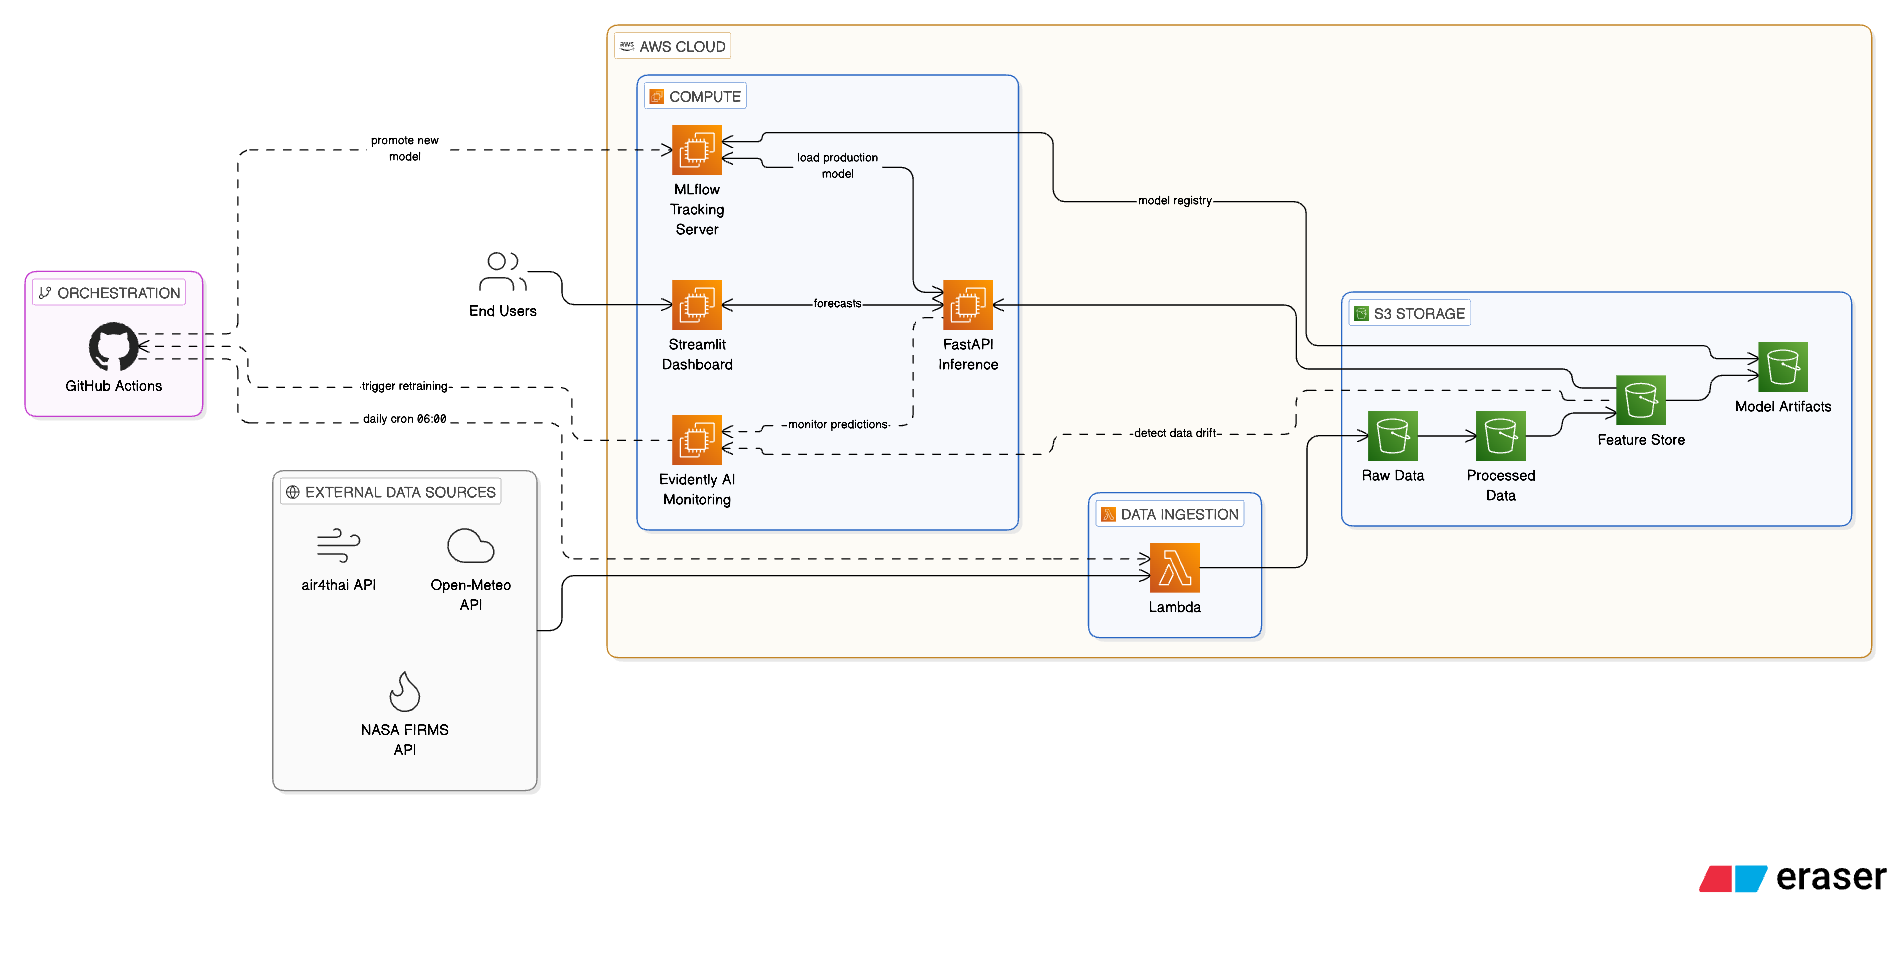
\includegraphics[width=\textwidth]{fig_cloud_architecture}
\caption{AWS cloud architecture for the ChiangMai Air Quality Alert System (CAAS). The pipeline spans three external data sources (air4thai API, Open-Meteo API, NASA FIRMS API), an AWS Lambda ingestion layer triggered daily at 06:00 UTC+7 via GitHub Actions, four S3 storage tiers (Raw, Processed, Feature Store, Model Artifacts), and a compute layer comprising MLflow Tracking Server, FastAPI Inference Server, Streamlit Dashboard, and Evidently AI drift monitoring. Dashed arrows indicate orchestration triggers and automated retraining signals.}
\label{fig:aws_architecture}
\end{figure}

\section{Storage Layers}

The storage architecture separates data by processing stage into four layers on Amazon S3:

\begin{itemize}
  \item \textbf{Raw Layer} (\texttt{s3://caas/raw/pm25/}, \texttt{raw/weather/}, \texttt{raw/fire/}) --- Immutable, append-only source data exactly as ingested. Files are never overwritten.
  \item \textbf{Processed Layer} (\texttt{s3://caas/processed/merged/}) --- Cleaned, validated, and schema-enforced daily merged files.
  \item \textbf{Feature Store} (\texttt{s3://caas/features/pm25\_daily\_chiangmai.csv}) --- ML-ready dataset with all 44 features and target columns, versioned by run date.
  \item \textbf{Model Artifacts} --- MLflow artifact store containing trained model files, hyperparameters, evaluation metrics, SHAP plots, confusion matrices, and loss curves per experiment run.
\end{itemize}

\section{MLOps Lifecycle}

\subsection{Experiment Tracking}

All training runs are logged to MLflow, recording: hyperparameters (learning rate, \texttt{n\_estimators}, LSTM units, sequence length, dropout rate), evaluation metrics (RMSE, MAE, $R^2$, Precision, Recall, F1, AUROC), artifacts (model file, feature importance plot, confusion matrix, loss curves), and the dataset version (snapshot date) used for training. This enables full reproducibility and direct side-by-side comparison between XGBoost and LSTM runs.

\subsection{Model Versioning and Promotion}

Models are managed through the MLflow Model Registry using a three-stage promotion workflow:
\[
\text{[Staging]} \;\longrightarrow\; \text{[Validation]} \;\longrightarrow\; \text{[Production]}
\]

\begin{itemize}
  \item \textbf{Staging} --- Newly trained model awaiting metric evaluation.
  \item \textbf{Validation} --- Model has passed RMSE and Recall thresholds; ready for deployment review.
  \item \textbf{Production} --- Currently serving model; only one model occupies this stage at any time.
\end{itemize}

Promotion to Production is automated when metrics pass predefined thresholds. Previous Production models are archived, not deleted, to enable rollback.

\begin{figure}[H]
\centering
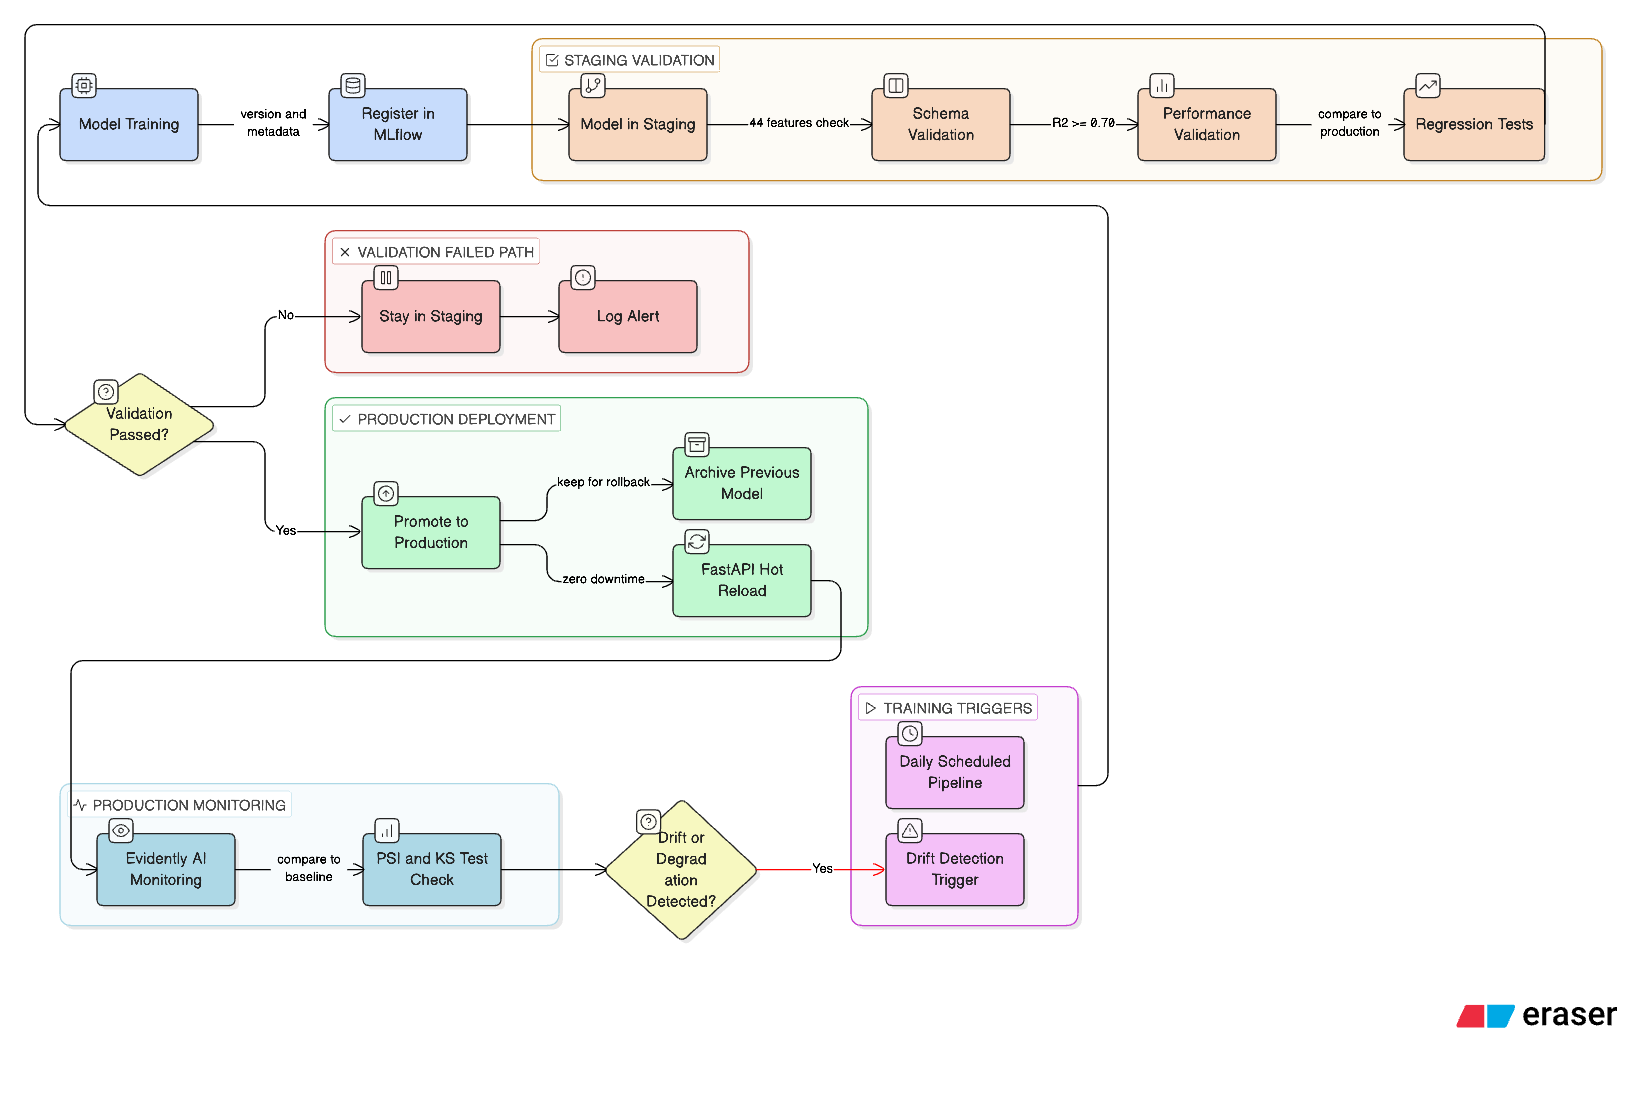
\includegraphics[width=\textwidth]{fig_model_promotion}
\caption{MLflow model promotion and lifecycle flow. Newly trained models are registered in MLflow and enter the Staging stage, where they undergo schema validation (44-feature check), performance validation ($R^2 \geq 0.70$), and regression tests against the current Production model. Failed validation keeps the model in Staging with an alert logged. On success, the model is promoted to Production with zero-downtime FastAPI hot-reload; the previous Production model is archived for rollback. Evidently AI drift detection and a daily scheduled pipeline serve as the primary retraining triggers.}
\label{fig:model_promotion}
\end{figure}

\subsection{Deployment Strategy}

The deployment architecture uses a hybrid batch and real-time API approach. The primary daily pipeline runs at 06:00 via GitHub Actions: it ingests the previous day's data, generates t+1/3/7 forecasts, and stores results to S3. A FastAPI service exposes \texttt{/predict} and \texttt{/alert} endpoints for the Streamlit dashboard and external consumers.

\begin{figure}[H]
\centering
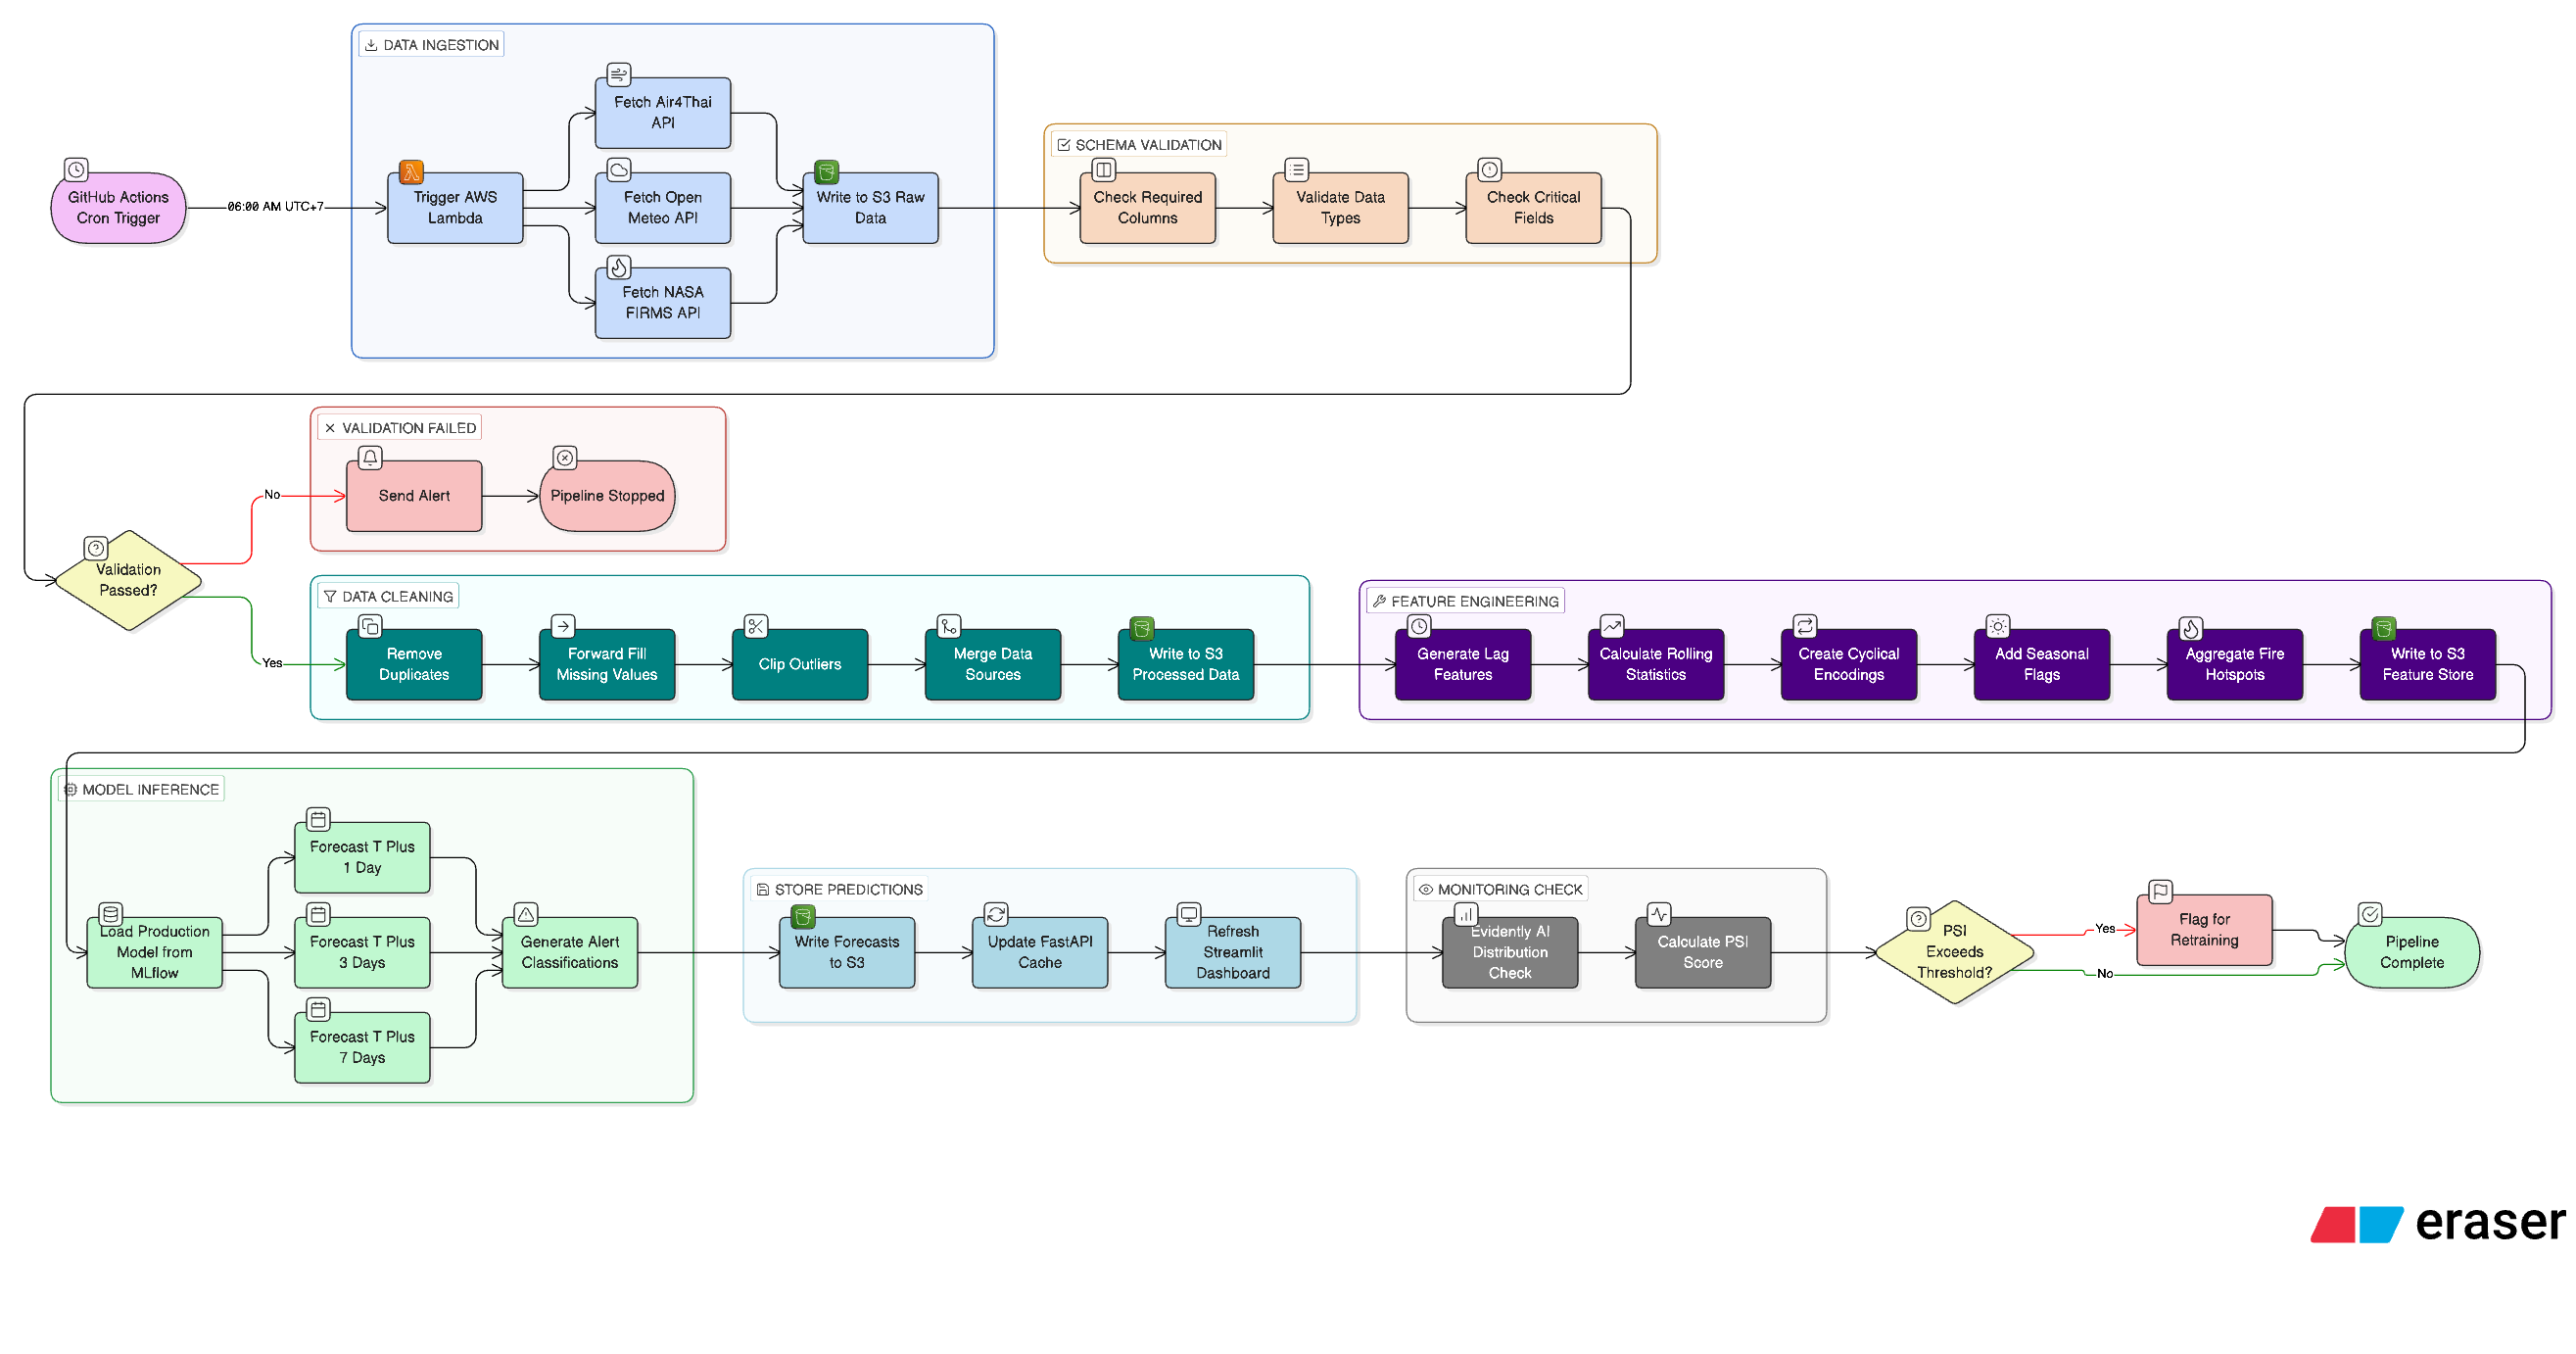
\includegraphics[width=\textwidth]{fig_daily_pipeline}
\caption{Daily MLOps pipeline execution flow triggered at 06:00~UTC+7 via GitHub Actions. The pipeline comprises seven stages: (1)~Data Ingestion via AWS Lambda fetching from air4thai, Open-Meteo, and NASA FIRMS APIs into S3 Raw; (2)~Schema Validation with a failure branch that sends an alert and stops the pipeline; (3)~Data Cleaning including duplicate removal, forward-fill for missing values, and outlier clipping; (4)~Feature Engineering producing 44 features (lag, rolling statistics, cyclical encodings, seasonal flags, fire hotspots) stored to S3 Feature Store; (5)~Model Inference generating PM2.5 regression values and alert-level classifications for t+1, t+3, and t+7 horizons; (6)~Store Predictions to S3 and update the FastAPI cache; (7)~Monitoring Check using Evidently AI PSI drift detection, flagging for retraining if PSI~$>$~0.2.}
\label{fig:pipeline_flow}
\end{figure}

\begin{figure}[H]
\centering
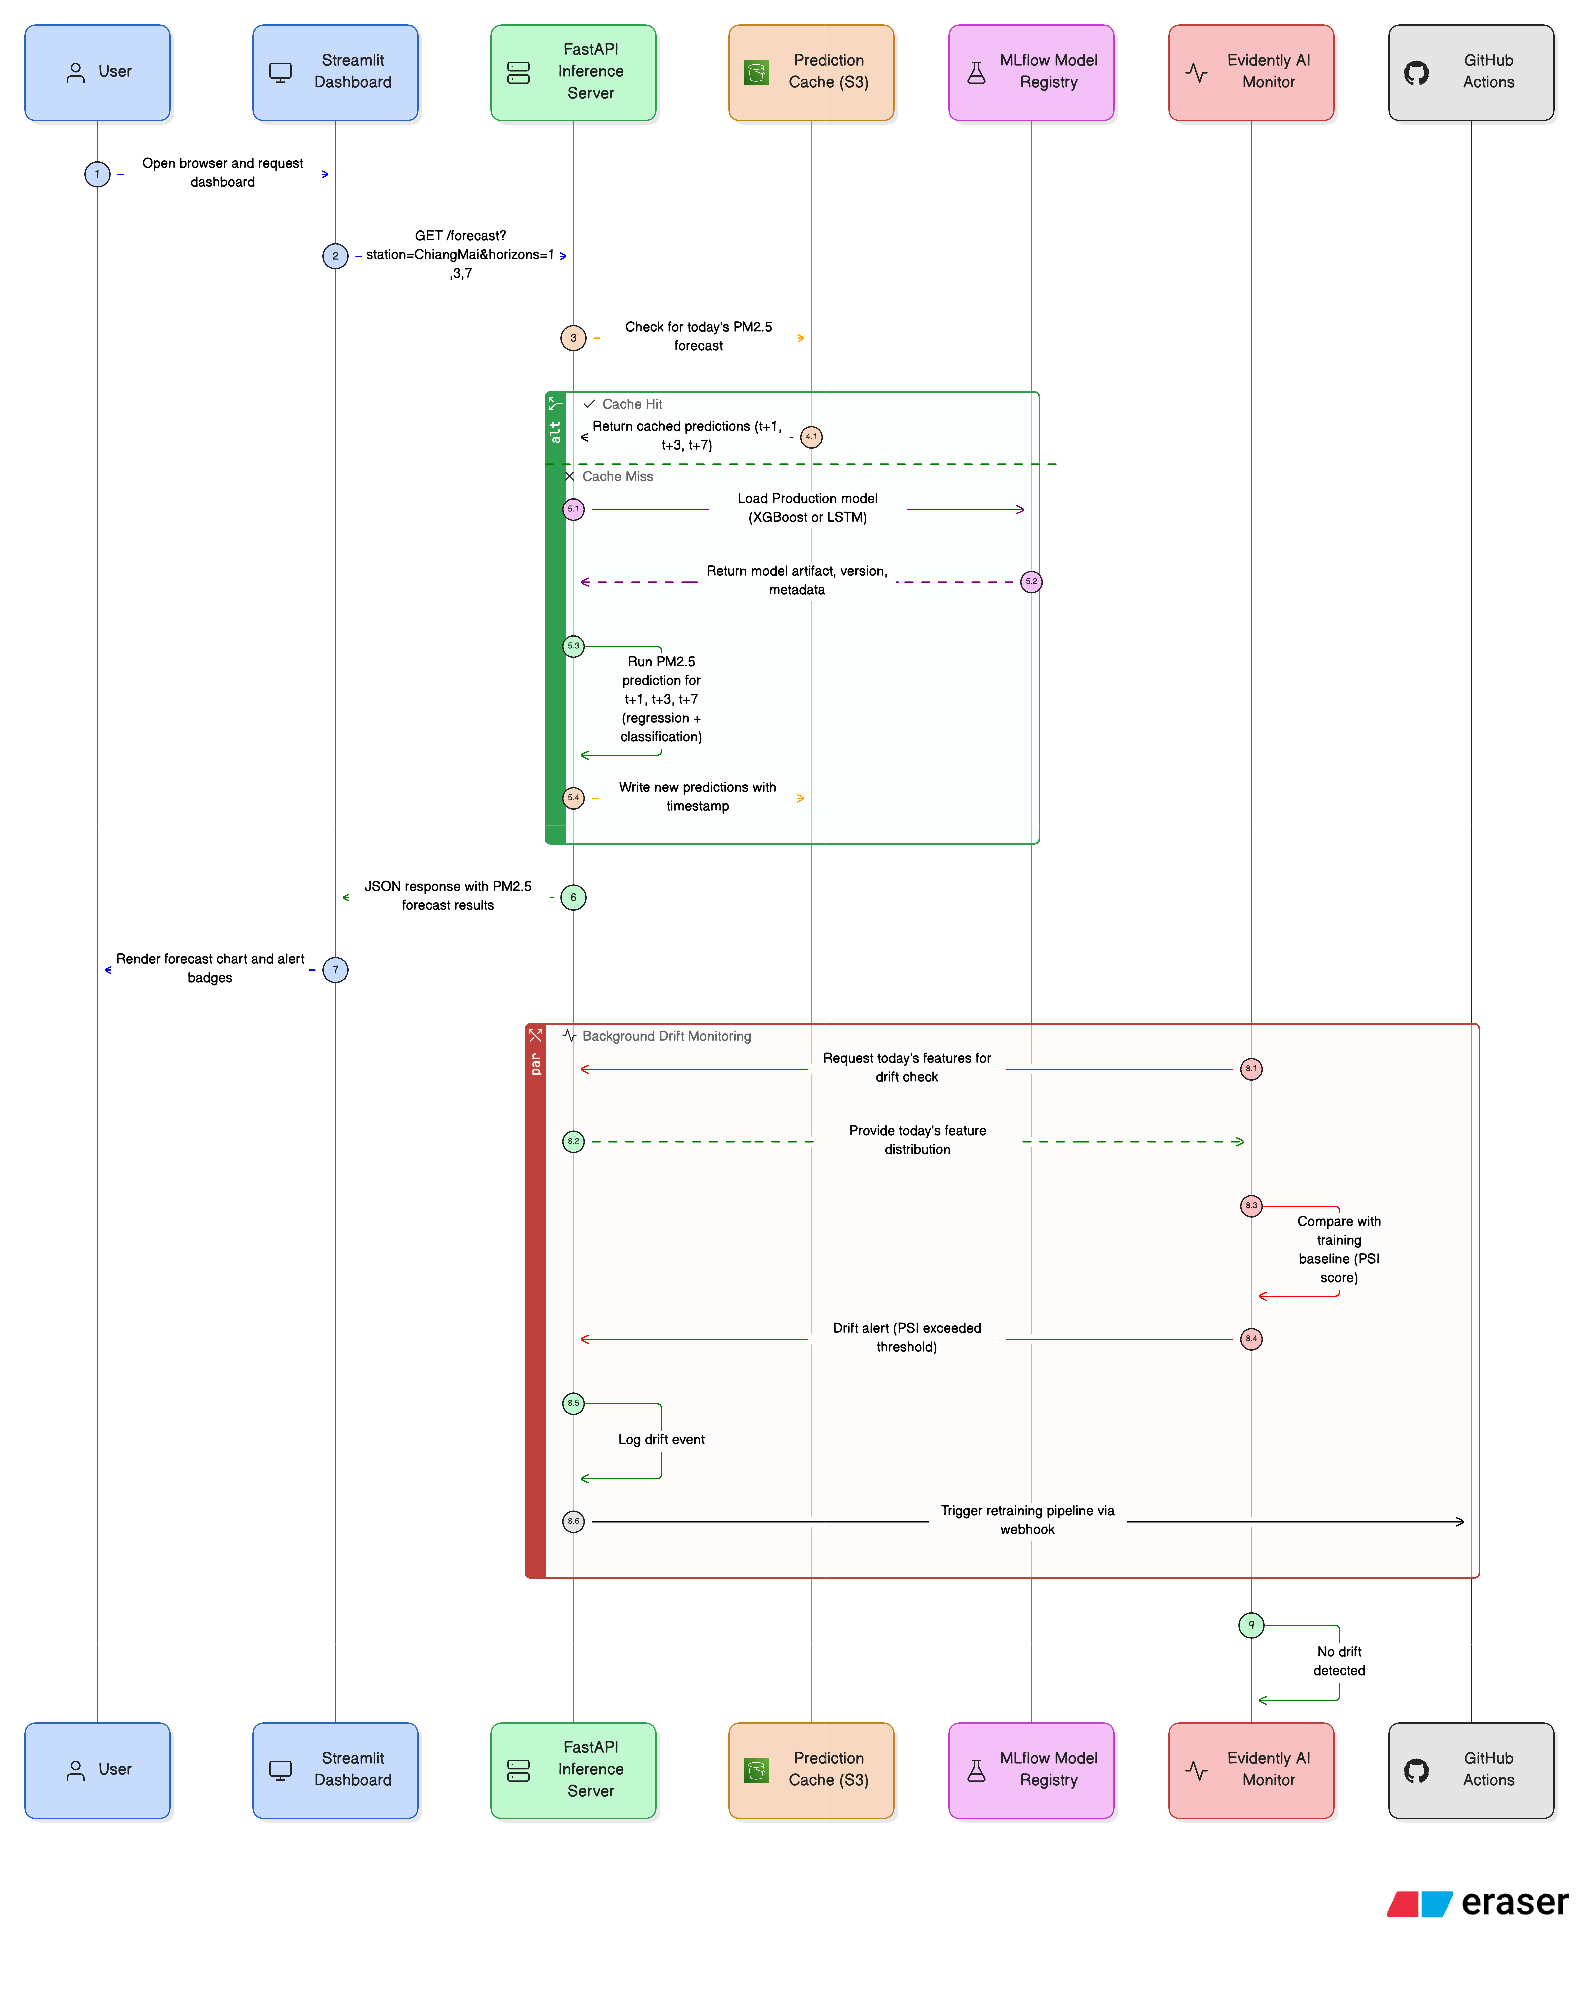
\includegraphics[width=0.92\textwidth]{fig_sequence_flow}
\caption[End-to-end PM2.5 forecast request flow for the CAAS system.]{End-to-end PM2.5 forecast request flow for the CAAS system. When a user opens the Streamlit Dashboard, it sends a \texttt{GET /forecast?station=ChiangMai\&horizons=1,3,7} request to the FastAPI Inference Server. The server first queries the S3 Prediction Cache: on a cache hit, predictions for t+1, t+3, and t+7 days are returned immediately; on a cache miss, the server loads the Production model from MLflow, runs PM2.5 regression and alert-level classification inference, writes the results to the cache, and returns a JSON response. In parallel, Evidently AI performs background drift monitoring by comparing today's feature distribution against the training baseline using PSI scoring. If PSI exceeds 0.2, a drift alert triggers the GitHub Actions retraining pipeline via webhook.}
\label{fig:sequence_flow}
\end{figure}

\section{Monitoring and Automated Retraining}

\subsection{Data Drift Monitoring}

Evidently AI generates weekly distribution comparison reports for key features (\texttt{PM25\_lag1}, \texttt{north\_avg\_PM25}, \texttt{wind\_speed}, \texttt{fire\_count}) using Population Stability Index (PSI) and Kolmogorov-Smirnov tests against the training data baseline. Drift scores exceeding defined thresholds are flagged for team review before any automated retraining decision.

\subsection{Model Performance Monitoring}

After each daily batch run, the previous day's PM2.5 prediction is compared against the now-known actual observation. A 7-day rolling RMSE and MAE are logged to MLflow. Automated retraining is triggered when:
\begin{itemize}
  \item Rolling RMSE exceeds 120\% of the training baseline, or
  \item The 30-day alert false negative rate exceeds 15\%.
\end{itemize}

Scheduled retraining also occurs in December each year, prior to the haze season, incorporating the most recent full year of data to reflect current environmental patterns.

\section{Infrastructure and Cost Estimate}

\begin{table}[H]
\centering
\caption{Estimated monthly AWS cloud infrastructure cost}
\label{tab:cost}
\begin{tabularx}{\textwidth}{@{}p{3cm}Xp{4cm}@{}}
\toprule
\textbf{Service} & \textbf{Usage} & \textbf{Est.\ Monthly Cost} \\
\midrule
Amazon S3           & 1--2~GB data + model artifacts            & \$0.03 \\
AWS Lambda          & Daily batch pipeline, $\sim$5~min/day     & \$0.00 (free tier) \\
EC2 t3.micro        & FastAPI serving + MLflow (always-on)      & \$7--8 (or \$0 with Learner Lab credits) \\
Open-Meteo API      & Daily weather fetch                       & \$0.00 (free) \\
NASA FIRMS API      & Daily fire data fetch                     & \$0.00 (free) \\
\midrule
\textbf{Total}      &                                           & \textbf{\$2--8/month} \\
\bottomrule
\end{tabularx}
\end{table}

The primary architectural trade-offs considered were: Lambda vs.\ EC2 for serving (Lambda is cheaper but introduces cold-start latency; EC2 provides consistent response time for the dashboard---EC2 chosen for serving, Lambda for batch only); and self-hosted MLflow vs.\ managed service (self-hosted on EC2 avoids additional managed service costs, acceptable at project scale).

\section{Data Quality Management}

Data quality is treated as a first-class concern in the pipeline. Each ingested record must pass schema validation before entering the processing layer; any violation halts the pipeline immediately with an explicit error log and GitHub Actions email notification. Silent failures are not permitted.

\subsection{Missing Value Handling Strategy}

\begin{table}[H]
\centering
\caption{Missing value handling by data source}
\label{tab:missing_values}
\begin{tabularx}{\textwidth}{@{}p{3cm}p{3.5cm}X@{}}
\toprule
\textbf{Source} & \textbf{Expected Missing Rate} & \textbf{Handling Strategy} \\
\midrule
air4thai PM2.5 (35T) &
  $\sim$2--3\% per year &
  Gaps $\leq$3 consecutive days: linear interpolation using adjacent lag and rolling mean values. Gaps $>$3 days: substitute 36T station data ($r = 0.94$). All imputed rows flagged with \texttt{is\_imputed = 1} column. \\[6pt]
Open-Meteo weather &
  Near zero (reanalysis data) &
  No action required; reanalysis fills missing observations by design. \\[6pt]
NASA FIRMS fire &
  Zero hotspots on some days is valid (not missing) &
  Fill \texttt{fire\_count = 0} and \texttt{fire\_frp\_sum = 0} on days with no detected hotspots in the bounding box. \\
\bottomrule
\end{tabularx}
\end{table}

\subsection{Schema Validation Rules}

Every pipeline run enforces the following validation checks before processing proceeds:
\begin{itemize}
  \item Expected column names and data types are present and correct.
  \item Date range is within bounds and contains no duplicate dates.
  \item Numeric values fall within physically plausible ranges (e.g., PM2.5 $\in [0, 500]$~\textmu g/m\textsuperscript{3}).
  \item Station identifiers match expected codes (35T, 36T).
\end{itemize}
Earlier PCD files (2011--2017) may differ in column count due to network expansion; the validator applies source-year-specific schemas to handle this gracefully.

\subsection{Pipeline Health Monitoring}

Each pipeline step (ingest $\to$ validate $\to$ preprocess $\to$ feature engineering $\to$ predict) emits structured logs containing: step name, timestamp, input row count, output row count, and pass/fail status. If any step fails, all downstream steps are blocked immediately. A data freshness check after each ingestion run verifies that the latest PM2.5 record date matches yesterday; if data is more than two days stale, the source is flagged as potentially unavailable and an alert is raised.

% ============================================================
%  CHAPTER 5 — EXPERIMENTAL PLAN AND EXPECTED CONTRIBUTIONS
% ============================================================
\chapter{EXPERIMENTAL PLAN AND EXPECTED CONTRIBUTIONS}

\section{Dataset Characteristics}

The training dataset comprises approximately 5,475 daily observations from 2011 to 2025, representing 15 complete annual cycles. Key statistical characteristics include:

\begin{itemize}
  \item \textbf{March 2025 average}: 55.1~\textmu g/m\textsuperscript{3} --- more than $3\times$ the WHO 24-hour guideline.
  \item \textbf{Single-day maximum}: 92.3~\textmu g/m\textsuperscript{3} (March 23, 2025).
  \item \textbf{Days exceeding Thailand's 25~\textmu g/m\textsuperscript{3} threshold}: 109 days (31\% of the year).
  \item \textbf{PM2.5 missing rate}: approximately 2--3\% per year.
  \item \textbf{Cross-station correlation} (35T vs.\ 36T): $r = 0.940$.
\end{itemize}

\section{Baseline Methods for Comparison}

Three strategies will be compared:

\begin{enumerate}
  \item \textbf{Persistence baseline} --- the forecast equals the most recent observed PM2.5 value (lag-1). This naive baseline establishes the lower bound that any model must exceed.
  \item \textbf{XGBoost with 44 engineered features} --- the primary tabular baseline described in Chapter~3.
  \item \textbf{LSTM with 30-day sequence window} --- the comparative sequential model.
\end{enumerate}

\section{Evaluation Metrics}

\begin{table}[H]
\centering
\caption{Evaluation metrics by task type and priority}
\label{tab:eval_metrics}
\begin{tabularx}{\textwidth}{@{}llX@{}}
\toprule
\textbf{Task} & \textbf{Metrics} & \textbf{Priority and Rationale} \\
\midrule
Regression (PM2.5 \textmu g/m\textsuperscript{3}) &
  RMSE, MAE, $R^2$ &
  RMSE is the primary regression metric; $R^2 \geq 0.70$ is the target benchmark. \\[6pt]
Classification (alert/no alert) &
  Precision, Recall, F1, AUROC &
  Recall is the primary classification metric. A missed true alert (false negative) carries greater public health cost than a false alarm (false positive). \\
\bottomrule
\end{tabularx}
\end{table}

\section{Experimental Setup}

Experiments will be conducted as follows:

\begin{enumerate}
  \item Both models trained on the 2011--2022 training set; hyperparameters tuned on the 2023 validation set using random search.
  \item Final evaluation on the 2024--2025 test set (fully unseen data).
  \item Separate experiments for each forecast horizon (t+1, t+3, t+7) to test whether any LSTM advantage is horizon-dependent.
  \item XGBoost SHAP analysis conducted to identify the most influential features for interpretability and domain insight.
  \item All runs logged to MLflow with full hyperparameter, metric, and artifact records for reproducibility.
\end{enumerate}

\section{Expected Contributions}

This project is expected to deliver the following contributions:

\begin{enumerate}
  \item \textbf{A production-ready MLOps pipeline for PM2.5 forecasting} demonstrating the full lifecycle from multi-source data ingestion to automated monitoring and retraining---applicable as a reference architecture for similar environmental monitoring systems.
  \item \textbf{An empirical comparison of XGBoost and LSTM} on a moderate-length daily environmental time series, providing evidence-based guidance on model selection for this class of problem.
  \item \textbf{A public-facing health alert dashboard} providing actionable advance warning to Chiang Mai residents during the haze season.
  \item \textbf{A reproducible multi-source feature engineering framework} integrating PM2.5 historical data, meteorological variables, and satellite fire detection into a unified ML-ready feature set.
\end{enumerate}

\section{Feasibility and Tool Selection}

All tools are open-source, well-documented, and either free or within Learner Lab credit limits. The technology stack is:

\begin{itemize}
  \item \textbf{Language}: Python 3.11
  \item \textbf{ML models}: XGBoost, TensorFlow/Keras (LSTM)
  \item \textbf{Experiment tracking}: MLflow
  \item \textbf{API serving}: FastAPI
  \item \textbf{Dashboard}: Streamlit
  \item \textbf{Drift monitoring}: Evidently AI
  \item \textbf{Orchestration / CI-CD}: GitHub Actions
  \item \textbf{Cloud}: AWS S3, Lambda, EC2 t3.micro (Learner Lab)
  \item \textbf{Data sources}: air4thai API (PCD), Open-Meteo API, NASA FIRMS API
\end{itemize}

The primary feasibility risk is LSTM training stability and overfitting given the dataset size. This risk is mitigated by the parallel XGBoost strategy: if LSTM proves problematic, XGBoost provides a fully capable production model.

\section{Team Roles and Responsibilities}

\begin{table}[H]
\centering
\caption{Team member roles and task ownership}
\label{tab:team_roles}
\begin{tabularx}{\textwidth}{@{}llX@{}}
\toprule
\textbf{Member} & \textbf{Student ID} & \textbf{Responsibilities} \\
\midrule
Supanut Kompayak &
  st126055 &
  Data pipeline design and implementation; feature engineering; model training (XGBoost + LSTM); experiment tracking (MLflow). \\[6pt]
Shuvam Shrestha &
  st125975 &
  FastAPI endpoint development; Streamlit dashboard;
  AWS cloud architecture design; cost estimation; CI/CD pipeline (GitHub Actions); Evidently AI monitoring setup; infrastructure deployment and maintenance. \\
\bottomrule
\end{tabularx}
\end{table}

\section{Known Limitations and Risk Mitigation}

Transparency about the project's limitations is essential for realistic feasibility assessment. Table~\ref{tab:risks} summarises the known risks and planned mitigations.

\begin{table}[H]
\centering
\caption{Known limitations and risk mitigation strategies}
\label{tab:risks}
\begin{tabularx}{\textwidth}{@{}lXX@{}}
\toprule
\textbf{Risk} & \textbf{Description} & \textbf{Mitigation} \\
\midrule
Dataset size for LSTM &
  5,475 daily observations is in the moderate-size regime where deep learning models are known to sometimes underperform well-tuned gradient boosting methods. &
  XGBoost serves as a fully capable fallback production model. Dropout and early stopping regularise LSTM. Results are reported honestly regardless of outcome. \\[6pt]

air4thai API access &
  The air4thai API (\texttt{air4thai.com}) is blocked outside Thai IP ranges, limiting automated ingestion from cloud infrastructure hosted outside Thailand. &
  Historical data (2011--2025) acquired via direct Excel file download. For ongoing ingestion, a lightweight script runs on a Thai IP (e.g., AIT campus) or via VPN, then pushes to S3. \\[6pt]

AWS Learner Lab expiry &
  Learner Lab credits may expire or reset during the semester, potentially disrupting always-on services. &
  All infrastructure is defined as code (GitHub Actions, configuration files) enabling rapid redeployment. MLflow and model artifacts are persisted to S3 to survive instance restarts. \\[6pt]

Concept drift &
  Long-term shifts in haze season onset, duration, and intensity due to climate change may cause model performance to degrade between training and future operational use. &
  Annual scheduled retraining in December each year incorporates the most recent full year of data to reflect current environmental patterns. \\[6pt]

Single-station dependency &
  If both 35T and 36T stations simultaneously experience extended outages, the pipeline has no PM2.5 source. &
  The data freshness check will raise an alert within 48~hours. Manual data acquisition from alternative PCD stations can be used as an emergency fallback. \\
\bottomrule
\end{tabularx}
\end{table}

\section{Project Timeline}

\begin{table}[H]
\centering
\caption{Project milestones and target dates}
\label{tab:timeline}
\begin{tabular}{@{}lll@{}}
\toprule
\textbf{Milestone} & \textbf{Owner} & \textbf{Target Date} \\
\midrule
Proposal submission & Both & March 12, 2026 \\
Full dataset ready (all years + weather + fire) & Supanut Kompayak & March 15, 2026 \\
XGBoost baseline trained and evaluated & Supanut Kompayak & March 15, 2026 \\
LSTM model trained and compared & Supanut Kompayak & March 22, 2026 \\
FastAPI + Streamlit dashboard deployed & Shuvam Shrestha & March 29, 2026 \\
AWS infrastructure + CI/CD operational & Shuvam Shrestha & March 29, 2026 \\
Monitoring and retraining pipeline live & Shuvam Shrestha & April 5, 2026 \\
Final report and presentation & Both & TBD \\
\bottomrule
\end{tabular}
\end{table}

% ============================================================
%  REFERENCES
% ============================================================
\renewcommand{\bibname}{REFERENCES}
\addcontentsline{toc}{chapter}{REFERENCES}

\begin{thebibliography}{99}

\bibitem{who2021}
World Health Organization (WHO). (2021).
\textit{WHO Global Air Quality Guidelines: Particulate Matter (PM2.5 and PM10), Ozone, Nitrogen Dioxide, Sulfur Dioxide and Carbon Monoxide}.
World Health Organization. Geneva.

\bibitem{seinfeld2016}
Seinfeld, J.~H., \& Pandis, S.~N. (2016).
\textit{Atmospheric Chemistry and Physics: From Air Pollution to Climate Change} (3rd~ed.).
John Wiley \& Sons, New Jersey.

\bibitem{liang2020}
Liang, Y., Ke, S., Zhang, J., Yi, X., \& Zheng, Y. (2018).
GeoMAN: Multi-level attention networks for geo-sensory time series prediction.
In \textit{Proceedings of the 27th International Joint Conference on Artificial Intelligence (IJCAI-18)},
pp.~3428--3434. AAAI Press.

\bibitem{chen2016xgboost}
Chen, T., \& Guestrin, C. (2016).
XGBoost: A scalable tree boosting system.
In \textit{Proceedings of the 22nd ACM SIGKDD International Conference on Knowledge Discovery and Data Mining},
pp.~785--794. ACM, New York.

\bibitem{hochreiter1997lstm}
Hochreiter, S., \& Schmidhuber, J. (1997).
Long short-term memory.
\textit{Neural Computation}, 9(8), 1735--1780.

\bibitem{makridakis2018m4}
Makridakis, S., Spiliotis, E., \& Assimakopoulos, V. (2018).
The M4 competition: Results, findings, conclusion and way forward.
\textit{International Journal of Forecasting}, 34(4), 802--808.

\bibitem{shwartzziv2022tabular}
Shwartz-Ziv, R., \& Armon, A. (2022).
Tabular data: Deep learning is not all you need.
\textit{Information Fusion}, 81, 84--90.

\bibitem{sculley2015}
Sculley, D., Holt, G., Golovin, D., Davydov, E., Phillips, T., Ebner, D.,
Chaudhary, V., Young, M., Crespo, J.-F., \& Dennison, D. (2015).
Hidden technical debt in machine learning systems.
In \textit{Advances in Neural Information Processing Systems (NeurIPS)}, 28.
Curran Associates.

\bibitem{zaharia2018mlflow}
Zaharia, M., Chen, A., Davidson, A., Ghodsi, A., Hong, S.~A., Murching, A.,
Nykodym, T., Ogilvie, P., Parkhe, M., Singh, A., Xie, C., \& Zumar, C. (2018).
Accelerating the machine learning lifecycle with MLflow.
\textit{IEEE Data Engineering Bulletin}, 41(4), 39--45.

\bibitem{pcd2024}
Pollution Control Department, Thailand. (2024).
\textit{Air Quality and Noise Management: Air4Thai Monitoring System}.
Retrieved from \url{http://air4thai.com}

\bibitem{firms2024}
NASA EOSDIS. (2024).
\textit{Fire Information for Resource Management System (FIRMS)}.
NASA Earthdata. Retrieved from \url{https://firms.modaps.eosdis.nasa.gov}

\bibitem{openmeteo2023}
Zippenfenig, P. (2023).
Open-Meteo.com Weather API.
\textit{Zenodo}. \url{https://doi.org/10.5281/zenodo.7970649}

\end{thebibliography}

\end{document}
